\section{CAN基础知识}

\subsection{CAN与LIN物理层的电平定义}
隐形状态和显性状态对应的CAN总线电平分别如表\ref{tab:rec_can_level}和\ref{tab:dom_can_level}所示:
% Table generated by Excel2LaTeX from sheet 'Sheet1'
\begin{table}[htbp]
    \centering
    \caption{隐形状态对应CAN总线电平}
      \begin{tabular}{lrrrl}
        \toprule
            & \multicolumn{1}{l}{min} & \multicolumn{1}{l}{典型值} & \multicolumn{1}{l}{max} & 单位 \\
        \midrule
      can H & 2     & 2.5   & 3     & v \\
      can L & 2     & 2.5   & 3     & v \\
      差分    & -50   & 0     & 50    & mv \\
      \bottomrule
      \end{tabular}%
    \label{tab:rec_can_level}%
\end{table}%
  
% Table generated by Excel2LaTeX from sheet 'Sheet1'
\begin{table}[htbp]
    \centering
    \caption{显形状态对应CAN总线电平}
      \begin{tabular}{lrrrl}
        \toprule
            & \multicolumn{1}{l}{min} & \multicolumn{1}{l}{典型值} & \multicolumn{1}{l}{max} & 单位 \\
        \midrule
      can H & 3     & 3.6   & 4.25  & v \\
      can L & 0.5   & 1.4   & 1.75  & v \\
      差分    & 1.5   & 2.25  & 3     & v \\
      \bottomrule
      \end{tabular}%
    \label{tab:dom_can_level}%
\end{table}%
  
Lin显性电平$V_{dom}<0.4(V_{bat}-0.6V)$,隐性电平$V_{rec}>0.4(V_{bat}-0.6V)$。

当电源电压$V_{bat}=12.5V$时,$V_{dom}<4.76V$,$V_{rec}>7.14V$。

\subsection{总线负载率计算}
标准数据帧的格式如图\ref{fig:can_frame}所示,
\begin{figure}[ht]
    \centering
    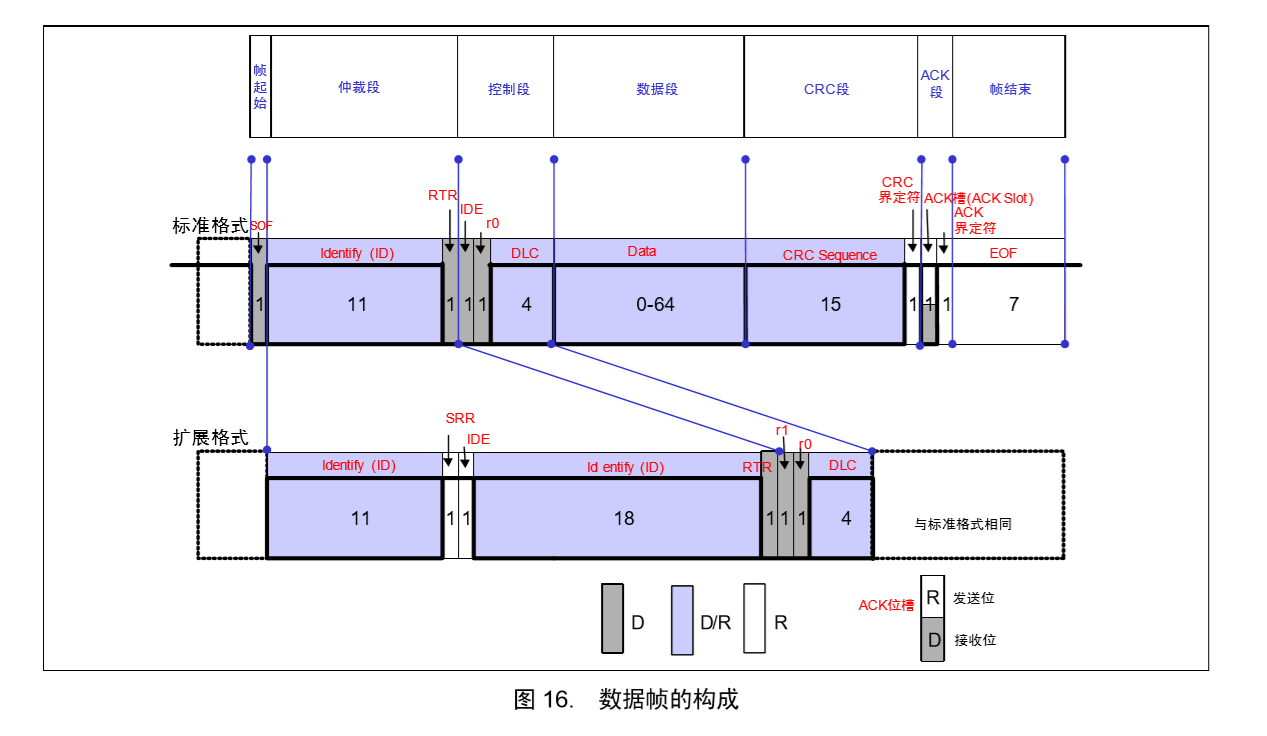
\includegraphics[scale=0.7]{pic/can_frame.png}
    \caption{CAN帧格式}
    \label{fig:can_frame}
\end{figure}

负载率由下式计算\cite{url_can_load_rate}:
$$lr = \frac{1000}{T} \frac{len_{frame}}{bdrate} $$
其中,$T$为数据帧的发送周期(ms),$len_{frame}$为数据帧的长度(单位,bit),$bdrate$为总线波特率。

由图\ref{fig:can_frame},可知,在不考虑位填充和帧间隔的情况下,一个数据帧的长度$len_{frame}=64+34+10=108$,
假定周期为10ms的帧及500kbps的波特率,总线负载可得$lr=0.0216=2.16\%$。

位填充:为防止突发错误而设定的功能。当同样的电平持续 5 位时则添加一个位的反型数据。 
位填充在帧的SOF~CRC段进行。因此最大情况下,位填充为$\frac{34+64}{5}=19$。

帧间隔如图\ref{fig:frame_jiange}所示。
\begin{figure}[ht]
    \centering
    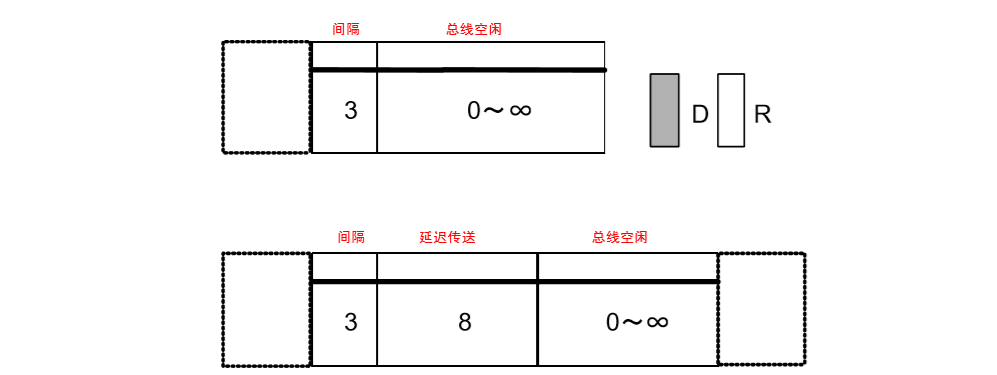
\includegraphics[scale=0.8]{pic/frame_jiange.png}
    \caption{帧间隔}
    \label{fig:frame_jiange}
\end{figure}
因此,最大帧长度$len_{frame}=34+64+10+19+3=130$,最大负载$lr=0.026=2.6\%$。



\subsection{网络系统开发中的相关文件}
网络配置文件包括:
\begin{enumerate}
    \item NRS文件:网络需要文档,主要定义了ECU的网络信号
    \item DBC LDF文件:CAN LIN的数据库文件
    \item fix net tgt文件:仅供使用网络基础软件模块的节点集成使用
\end{enumerate}
EP阶段,在整网所有节点信号需求锁定后,5周内要释放所有的网络配置文件。

\subsection{网络休眠与网络故障}
网络休眠:
\begin{enumerate}
    \item ub\_keepnetwork:
    
    当所有从节点都没有网络通信需求时,各自的ub\_keepnetwork=0,此后主节点延时一段时间后,发送shutdown控制网络休眠
    \item ub\_wakenetwork:
    
    当任一从节点有网络通信需求时,ub\_wakenetwork=1,唤醒主节点,主节点在唤醒整个网络
\end{enumerate}

网络故障:
\begin{enumerate}
    \item busoff:当一个节点无法发送报文时,即该节点发生busoff,而不是网络busoff
    \item node missing:处于同一网络的节点接收不到其它节点的报文时,记录其他节点node missing
\end{enumerate}

\subsection{各路CAN的定义与说明}
在公司网络总线中,相关的几路CAN总线定义如下表\ref{tab:canbus_def}所示:
% Table generated by Excel2LaTeX from sheet 'Sheet1'
\begin{table}[htbp]
    \centering
    \caption{几路CAN总线定义}
      \begin{tabular}{llllll}
      \toprule
      spy 名称 & DBC文件 & 对应CAN名称 & 高低CAN序号 & dlc   & 工具 \\
      \midrule
      HS CAN & CAN1  & PT    & 6 14  & dlc2  & spy \\
      MS CAN & CAN2  & CH    & 12 13 & dlc2  & spy \\
      HS CAN2 3G & CAN3  & Body  & 3 11  & dlc2  & spy \\
      HS CAN3 3G & CAN4  & info  & 1 9   & dlc2  & spy \\
      ?     & CAN6  & hybrid & 2 10  & dlc2  & spy \\
      ?     & ?     & diagcan & 6 14  & dlc1  & eds \\
      \bottomrule
      \end{tabular}%
    \label{tab:canbus_def}%
  \end{table}%
    
